\section{Background and Motivation}
\label{sec:bg}

In this section we focus on the DNP3 transactions the paper covers, the features that leak from
them and how an adversary uses them in fingerprinting, and the opportunity that a programmable
data plane gives us to change the timing without touching the endpoints.

\begin{figure}[t]
\centering
\IfFileExists{figures/fig_ladder.pdf}{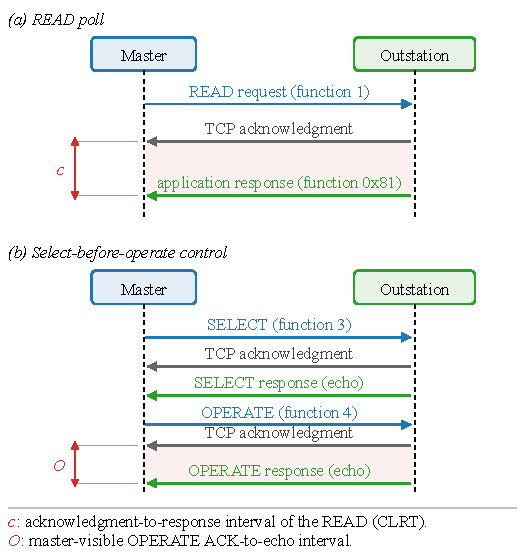
\includegraphics{figures/fig_ladder}}{\figplaceholder{DNP3 transaction ladder: (a) READ request, TCP ACK, application response; (b) SELECT, TCP ACK, SELECT response, OPERATE, TCP ACK, OPERATE response.}}
\caption{The DNP3 transactions the paper measures, as seen on the master-facing link; requests in
blue, transport-layer acknowledgments in grey, and application responses in green. (a) A READ
poll: the request, the outstation's transport-layer acknowledgment, and its application-layer
response. The interval $c$ between the acknowledgment and the response is the cross-layer
response time (CLRT). (b) A select-before-operate control: SELECT and OPERATE each produce an
acknowledgment and a solicited application response. The interval $O$ between the OPERATE's
acknowledgment and its solicited response is the master-visible OPERATE response-to-ACK interval.}
\label{fig:ladder}
\end{figure}

\textbf{The DNP3 read and control transactions.} DNP3 carries supervisory control and data
acquisition (SCADA) traffic over TCP between a master and an outstation~\cite{ieeeIEEEStandardElectric2012}.
The master polls the outstation with a READ request (function code 1), and the outstation
returns the requested measurements in an application-layer response (function code 0x81). A
control command, on the other hand, uses select-before-operate (SBO): the master first sends a
SELECT (function code 3) that names an output point, and the outstation returns a SELECT
application response; the master then sends an OPERATE (function code 4), which the outstation
confirms with a solicited OPERATE application response. A DNP3 control response repeats the
control object, but it is a solicited application response, not a distinct message type. Because DNP3 runs over TCP, every request is also
acknowledged at the transport layer before the application answers. As such, each transaction on
the wire is a request, a TCP acknowledgment that carries no DNP3 payload, and a DNP3 response, in
that order, as Figure~\ref{fig:ladder} shows. We use these terms consistently in the rest of the
paper: the acknowledgment is the TCP segment with the ACK flag that the outstation returns
first, and the response is the DNP3 application frame that follows it.

\textbf{Why the transaction timing is a fingerprint.} The acknowledgment is produced by the
outstation's TCP stack as soon as the request arrives, whereas the response is produced by its
application only after the device has done the work the request asks for. Consequently, the
interval between the two, the CLRT, reflects the outstation's internal processing rather than
the network path, and it differs between device models and between the kinds of work they do.
Formby et al.\ used it to tell device types and models apart in a substation network, and used
the time a device takes to complete a control operation as a second feature that reveals the
physical device behind the command~\cite{formbyWhosControlYour2016}. Our own measurements on a
physical SEL-751A relay show the same effect on one device: with no timing defense, the median
CLRT is 2.116~ms for a READ, 2.050~ms for a SELECT and 2.937~ms for an OPERATE, each with a long
tail, so the three transaction classes are already partly separable from timing alone
(Section~\ref{sec:eval}).
The function codes remain visible in the plaintext, so the classes themselves are not a secret;
what the timing adds is a channel that identifies the device and its operation without any
payload, and that survives encryption.

\textbf{Measured and inferred events.} Everything the paper measures is a packet timestamp on the
master-facing link, i.e., the request, the acknowledgment, and the response. The switch-internal
release times and any event on the relay-facing link are not observed; where the paper names
them, they are inferred from the configuration. Physical breaker motion is never measured.

\textbf{Programmable data planes.} A programmable switch exposes a match-action pipeline, written
in P4~\cite{bosshartP4ProgrammingProtocolIndependent2014}, that parses headers, keeps per-packet
state in registers, and places packets into output queues at line rate. Because such a pipeline can delay and release a packet
without a host in the loop, it can hold an outstation's acknowledgment and response and release
them on a schedule that the operator sets, while changing no endpoint and no byte of the payload.
